% Chapter Template

\chapter{Numerical analysis} % Main chapter title
\label{NumAnalysis} % Change X to a consecutive number; for referencing this chapter elsewhere, use \ref{ChapterX}

%----------------------------------------------------------------------------------------
%	SECTION 1
%----------------------------------------------------------------------------------------

\section{Theoretical preparation}

In order, to prepare the treatment of cracks experiments, many details must be examined.
%----------------------------------------------------------------------------------------
%	SUBSECTION 1
%----------------------------------------------------------------------------------------

\subsection{Abaqus modelization}

First, the purpose of this work is to compare the behavior of wood species with numerical analysis. That is why the preparation work begin by the modelisation of MMCG specimen on Abaqus software. Abaqus allows to model a specimen, create a mesh, adapted to the geometry, initialize a crack, and obtain data from a virtual crack.

The creation of the specimen follows the MMCG geometry specimen. It is explained in \parencite{Reference7} thesis. The precrack has a length of 25mm. 2D and 3D models were created. A 2.9mm line was put to continue the precrack and represent the cutter precrack done experimentally.

Abaqus allows to create a material by adding his characteristics. In wood case as it is studied in this work, orthotropic characteristics must be inquired. Abaqus asks for a D matrix defined as in \ref{eq:D matrix}
\begin{equation}
	\left[
	\begin{array}{rrrrrr}
		D_{1111} & D_{1122} & D_{1133} &
		0 & 0 & 0 \\
		D_{1122} &
		D_{2222} &
		D_{2233} &
		0 & 0 & 0 \\
		D_{1133} &
		D_{2233} &
		D_{3333} &
		0 & 0 & 0 \\
		0 & 0 & 0 &
		D_{1212} & 0 & 0 \\
		0 & 0 & 0 & 0 &
		D_{1313} & 0 \\
		0 & 0 & 0 & 0 & 0 &
		D_{2323} \\
	\end{array}
	\right]
	with : \\
	\\
	\left\{
	\begin{array}{lllll}
		D_{1111}=E_{1}(1-\nu_{23}\nu_{32})\gamma \\
		D_{2222}=E_{2}(1-\nu_{13}\nu_{31})\gamma \\
		D_{3333}=E_{3}(1-\nu_{12}\nu_{21})\gamma \\
		D_{1122}=E_{1}(\nu_{21}+\nu_{31}\nu_{23})\gamma \\	D_{1133}=E_{1}(\nu_{31}+\nu_{21}\nu_{32})\gamma	 \\	D_{2233}=E_{2}(\nu_{32}+\nu_{12}\nu_{31})\gamma \\	D_{1212}=G_{12} \\	D_{1313}=G_{13} \\	D_{2323}=G_{23} \\
	\end{array}
	\right.
	\label{eq:D matrix}
\end{equation}
It means that it is necessary before using ABAQUS to determine all these coefficients depending on the specie and the direction of the wood. These values for specimen at 12\% of MC which are the shearing $G_{ij}$ and longitudinal modulus $E_{i}$, the Poisson's coefficient $\nu_{ij}$ and $\gamma$ change for each species. After filling this D matrix it is possible to characterize the material of the specimen modelized. As an example, Okoume specie can be characterized by the values in \ref{eq:Okoume physicals values} which are confirmed by \parencite{Reference5}
\begin{equation}
	\left\{
	\begin{array}{llllllllllll}
		E_{1} = 9634 (MPa) \\
		E_{2} = 1090 (MPa)\\
		E_{3} = 522 (MPa) \\
		\nu_{12} = 0,369 \\
		\nu_{13} = 0,472 \\
		\nu_{23} = 0,705 \\
		\nu_{21} = \nu_{12}\dfrac{E_{2}}{E_{1}} = 0,042 \\
		\nu_{31} = \nu_{13}\dfrac{E_{3}}{E_{1}} = 0,026 \\
		\nu_{32} = \nu_{23}\dfrac{E_{3}}{E_{2}} = 0,338 \\
		G_{12} = 808 (MPa) \\
		G_{13} = 594 (MPa) \\
		G_{23} = 186 (MPa) \\
		\gamma = \dfrac{1}{1-\nu_{12}\nu_{21}-\nu_{13}\nu_{31}-\nu_{23}\nu_{32}-2\nu_{21}\nu_{32}\nu_{13}} = 1,387 \\
	\end{array}
	\right.
	\label{eq:Okoume physicals values}
\end{equation}
These values can evolve due to temperature and relative humidity. This is why, Guitard's model from \parencite{Reference2} are used. Indeed, by knowing the temperature, the relative humidity and the volumic weight of a specimen, it is possible to obtain at least nine of the physicals values presented in \ref{eq:Okoume physicals values}. An important factor to obtain these parameters is also the wood type, harwood or softwood.

Load and Boundaries Conditions (BC) must be also inquired. In 2 dimensions, the specimen was considered as blocked from one of the upper side. While the load is applied on the other upper side, even if the applied load is a surface one, localized in the hole as the BC. In 3 dimensions, load and BC are applied in the holes, so it must be closer to experimental conditions. The BC was considered as an embedding, even if in experimental conditions a displacement can occurs on the pin. The magnitude was chosen as :

Concerning the mesh, it is special on this geometry. But it will be focused on the crack and around it. The interest is to determine the displacement and the strain applied on the element of the mesh. That is why a ZOI was created \ref{fig:Fig16} and a thinner mesh was done in this area. Indeed, it is the interesting one, where the crack must develop.
\begin{figure}[h]
	\centering
	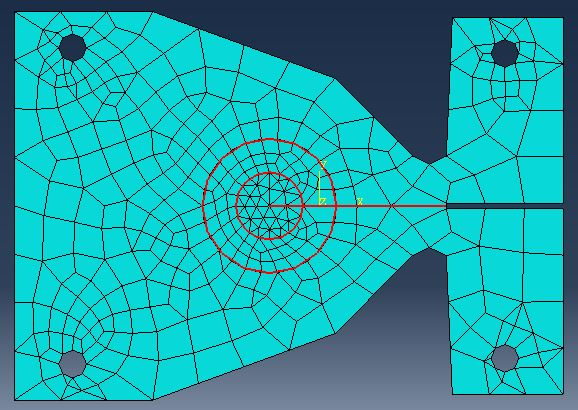
\includegraphics[scale=0.5]{Figures/Abaqus_Screenshot}
	\decoRule
	\caption[ABAQUS 2D specimen]{ABAQUS 2D Okoume specimen meshed with underlined ZOI and crack direction.}
	\label{fig:Fig16}
\end{figure}
Then, a step is created and also a job with the crack developement. This job allows to obtain a representation of the strain in each element of the mesh.



TO DEVELOP